\documentclass[xcolor=table]{beamer}
\usepackage[utf8]{inputenc}
\usepackage[francais]{babel}
%\usetheme{Boadilla}
%\usecolortheme{rose}
%\usecolortheme{crane}
\usefonttheme{structuresmallcapsserif}
\setbeamertemplate{navigation symbols}{}

\definecolor{Main}{rgb}{0.74, 0.13, 0.19}
\definecolor{Accent1}{rgb}{0.76,0.36,0.13}
\definecolor{Accent2}{rgb}{0.54,0.1,0.4}

\usecolortheme{rose}
%\useinnertheme[shadow]{circles}
\usecolortheme{whale}
%\useoutertheme{infolines}

\usecolortheme[named=Accent1]{structure}

\setbeamercolor{alerted text}{fg=Accent2}
%\setbeamercolor{palette primary}{fg=white}
%\setbeamercolor{palette secondary}{bg=Accent1}
%\setbeamercolor{palette tertiary}{bg=Accent2,fg=white}


\setbeamerfont{page number in head/foot}{size=\large}
\setbeamercolor{page number in head/foot}{fg=Main}
% page/total
%\setbeamertemplate{footline}[frame number]
% pas de total
\setbeamertemplate{footline}{%
    	\hfill%
	\usebeamercolor[fg]{page number in head/foot}%
	\usebeamerfont{page number in head/foot}%
	\insertframenumber\kern1em\vskip2pt%
}

\setbeamersize{text margin left=1em}
\setbeamersize{text margin right=1em}

%font
\usepackage[T1]{fontenc}
\usepackage[oldstylenums]{kpfonts}


%proper math and math symbols
%\usepackage{amsmath}
\usepackage{amssymb}

\usepackage{datenumber,fp}

\usepackage{siunitx}

\usepackage{tabu}
\usepackage{multirow}
\usepackage{booktabs}

% Allow the usage of graphics (.jpg, .png, etc.) in the document
\usepackage{graphicx}
\usepackage{tikz}
\usetikzlibrary{arrows,shapes,backgrounds, calc, positioning, topaths,chains, intersections, decorations.markings, shapes.geometric, matrix,patterns,mindmap}
%\usetikzlibrary{positioning, patterns,topaths,chains,matrix}

\usepackage{pgfplots}
\usepgfplotslibrary{groupplots}
\usepgfplotslibrary{external}



%beamer related package

\usepackage{todonotes}
\presetkeys{todonotes}{inline}{}


%bibliography
\usepackage[style=authoryear-comp, language=british,eprint=false, url=false, doi=false, sortcites=true, sorting=none, isbn=false, firstinits=true,maxcitenames=6]{biblatex}
%minimal citations
\AtEveryCitekey{%
	\clearfield{title}
	\clearfield{pages}
	\clearfield{volume}
	\clearfield{number}
	\clearfield{month}}
\newcommand{\myfullcite}[1]{{\scriptsize\fullcite{#1}}}
\renewbibmacro{in:}{%
  \ifentrytype{article}{}{%
  \printtext{\bibstring{in}\intitlepunct}}}
%\bibliography{biblio}


\newcolumntype{P}[1]{>{\raggedright}p{#1}}

\institute[E.N.S. Lyon]{Laboratoire de physique, Ecole Normale Supérieure de Lyon}
\title[Yoghurt under stress]{Yoghurt under stress}
\author[M. Leocmach]{Mathieu Leocmach}
\date{1st June 2014}


\begin{document}
\tikzset{every mark/.append style={scale=0.8}}
\pgfplotsset{compat=1.3, every axis/.append style={footnotesize}}

\AtBeginSection[]{
	\addtocounter{framenumber}{-1}
	\begin{frame}[plain]
		\tableofcontents[currentsection, hideothersubsections]
	\end{frame}
}

\begin{frame}[plain]
	\titlepage
\end{frame}

\setcounter{framenumber}{0}


\begin{frame}{Application of biogels}
\begin{tabu}{cX[c]c}
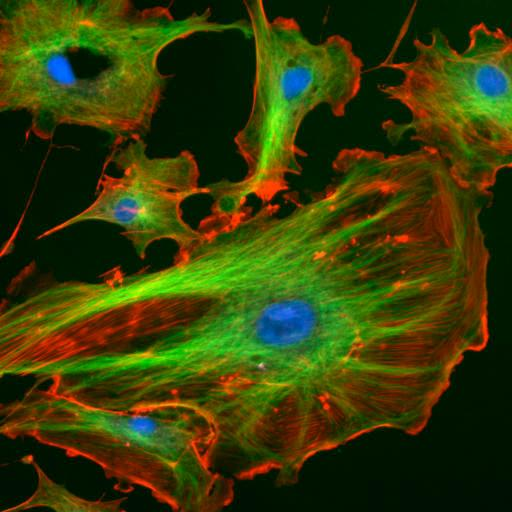
\includegraphics[height=0.3\textheight]{cell_mech} &
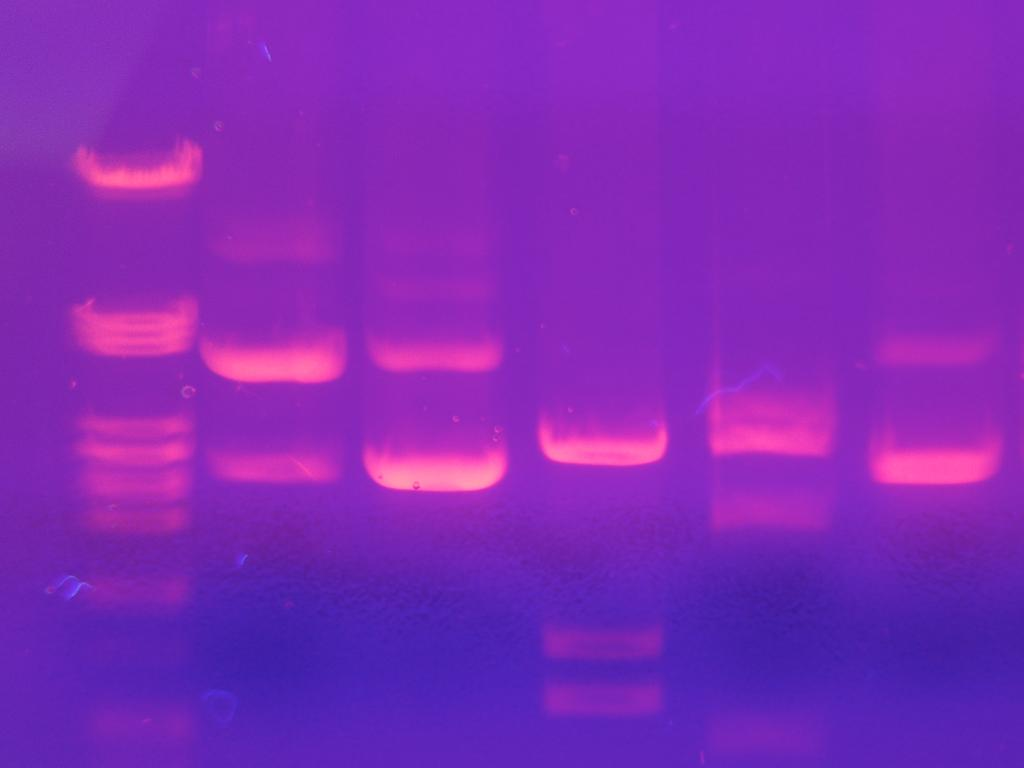
\includegraphics[height=0.3\textheight]{electrophoresis} &
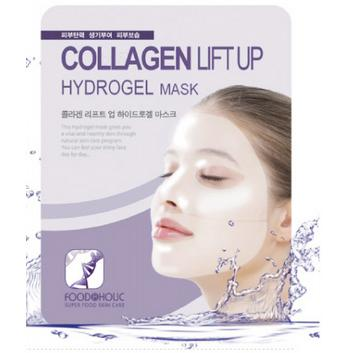
\includegraphics[height=0.3\textheight]{cosmetics} \\
Cell mechanics & Electrophoresis & Cosmetics\\
\end{tabu}
\begin{tabu}{X[c]X[c]}
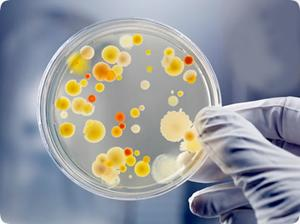
\includegraphics[height=0.3\textheight]{bacterial_culture} &
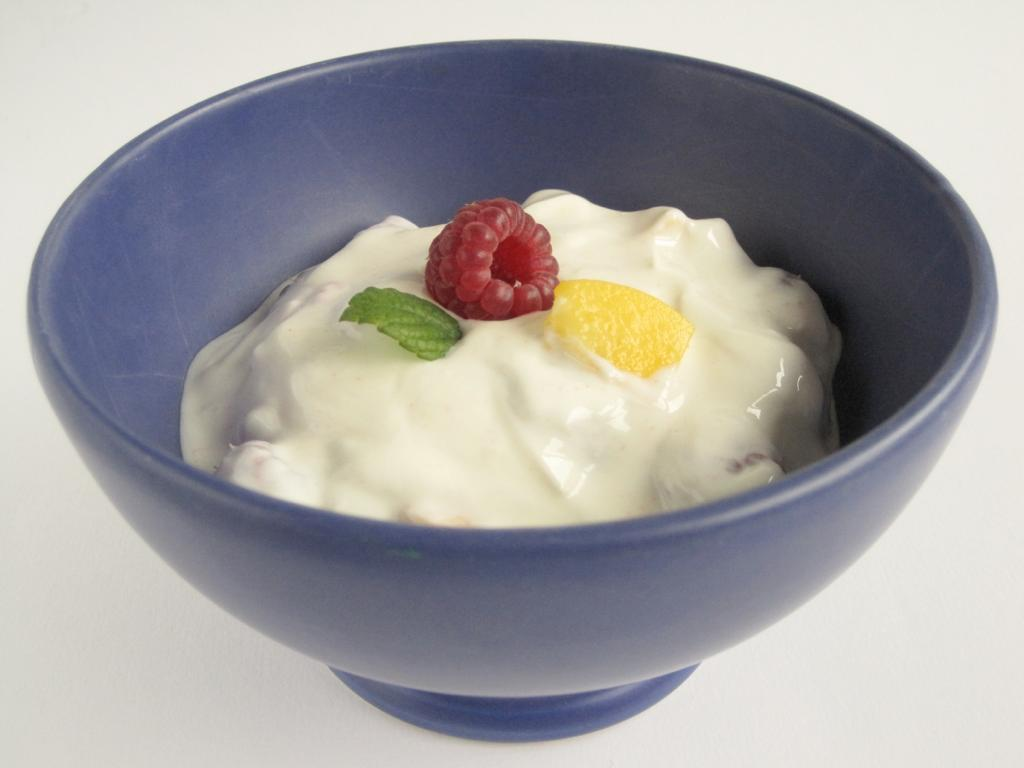
\includegraphics[height=0.3\textheight]{food} \\
Bacterial culture & Food\\
\end{tabu}

\begin{footnotesize}
\begin{block}{Sources}
\begin{tabu}{lXl}
Wikimedia Commons & www.madaboutscience.com & www.keautystore.com\\
\end{tabu}
\end{block}
\end{footnotesize}
\end{frame}



\begin{frame}{Fundamental issues in biogels}
\begin{itemize}
\item Linear elasticity in not well understood \textit{\scriptsize Gardel et al. Science 2004}
\item Strain and stress stiffening \textit{\scriptsize Storm et al. Nature 2005}
\item Fractures \textit{\scriptsize Bonn et al. Science 1998, Baumberger et al. Nature Material 2006}
\item Mechanical instabilities and morphogenesis \textit{\scriptsize Shyer et al. Science 2013}
\end{itemize}
\begin{block}{Our questions}
\begin{itemize}
\item What is the behaviour of a biogel under shear deep into the nonlinear regime?
\item What is the role of the solvent in mechanical instabilities?
\end{itemize}
\end{block}
\end{frame}

\section{Our system: Yoghurt}

\begin{frame}{Acid-set protein gel}
\begin{block}{Recipe}
\begin{itemize}
\item Water (\SI{30}{\celsius})
\item Sodium caseinate (milk protein) 4\%
\raisebox{0.6\normalbaselineskip}[0pt][0pt]{$\left.\rule{0pt}{1.1\normalbaselineskip}\right\}$ stable solution}
\item Glucono-$\delta$-lactone (GDL) 1\% $\Rightarrow$ slow acidification
\end{itemize}
\end{block}

\begin{columns}
\column{0.5\textwidth}
\begin{tikzpicture}
	\begin{groupplot}[%
		group style={
			group name=g, group size=1 by 2,
			xticklabels at=edge bottom,
			vertical sep=0,
			},
		xmode=log,
		xmin=1e2,xmax=3e5,
		scale only axis,
		width=\textwidth-4em,
		height=0.3\textwidth,
		extra tick style={grid=major},%
		ylabel absolute, every axis y label/.append style={anchor=base, yshift=-0.5em}
		]
	\nextgroupplot[
		ymin=0, ymax=7, ylabel={pH},
		%extra y ticks={4.6}, extra y tick labels={},%
		]
	\addplot+[no marks,Accent2] table{Y190_cas4_gdl1.pH};
	\draw[help lines] (axis cs:1e2,4.6) -- (axis cs:1.3979e4,4.6) node[pos=0, below right, font=\scriptsize, text width=0.4\textwidth] {isoelectric point $pH\approx 4.6$}  -- (axis cs:1.3979e4,0);
	

	\nextgroupplot[
		xlabel={time (s)},
		ymin=0, ylabel={$\textcolor{Accent2}{G^\prime}, \textcolor{Main}{G^{\prime\prime}}$ (\si{\pascal})},
		extra x ticks={1e5}, extra x tick labels={},
		]
	\addplot+[no marks,Accent2] table{cas4_GDL1_Y22.prise};
	\addplot+[no marks,Main] table[y index=2]{cas4_GDL1_Y22.prise};
	\begin{scope}[font=\scriptsize]
		\node[above right] at (rel axis cs:0,0) {casein ``micelles''};
		\draw[<-] (axis cs:1.3979e4,654) -- +(-1em,0) node[left] {gelation};
	\end{scope}
	\end{groupplot}
\end{tikzpicture}

\column{0.5\textwidth}
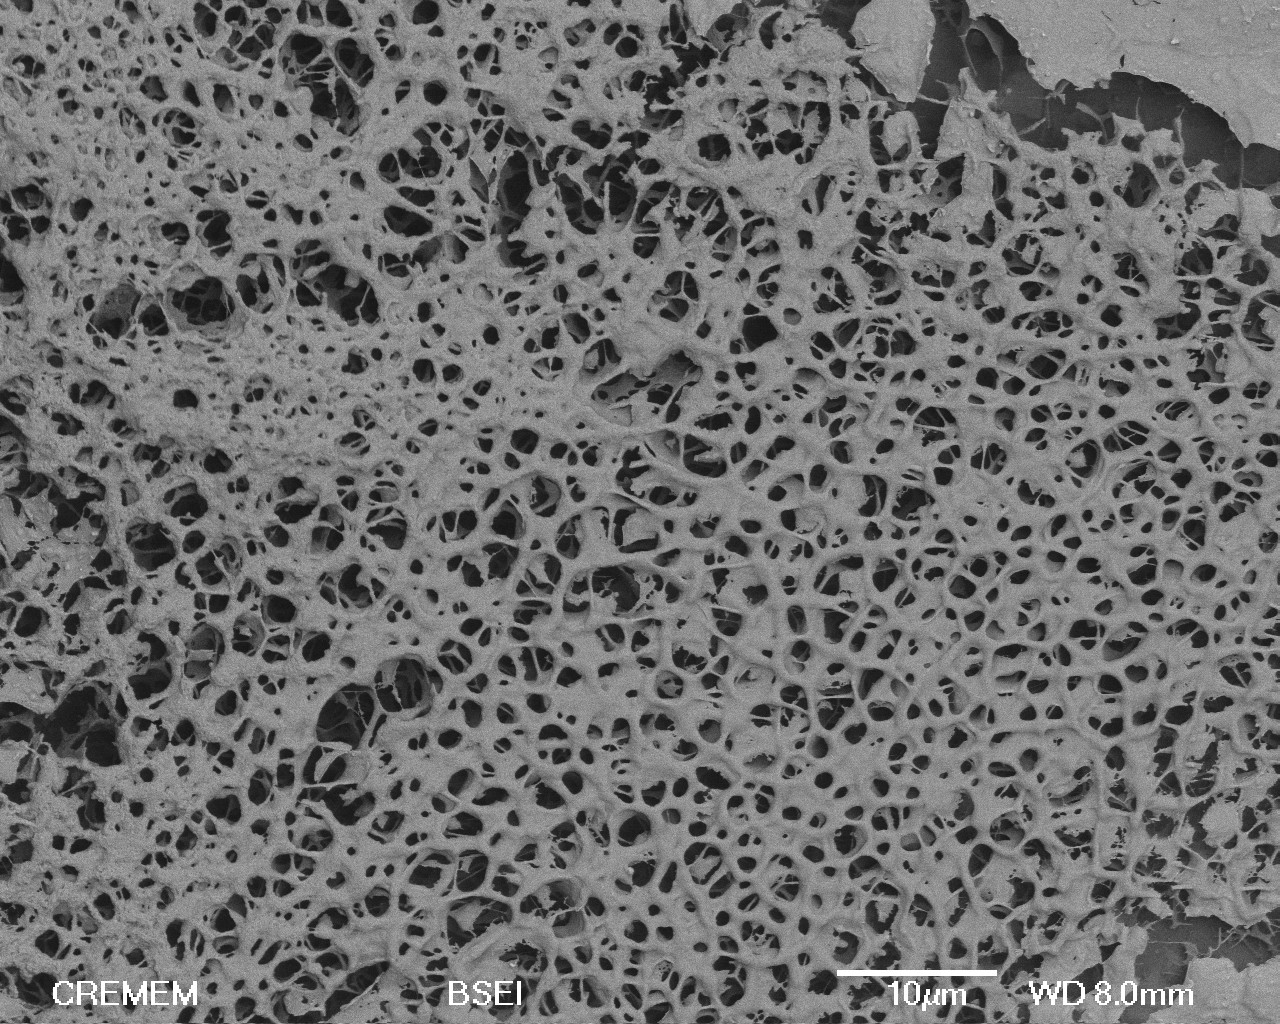
\includegraphics[width=\textwidth, clip=true, trim=0 0 0 10cm]{MEB_cas4_gdl1_22}

\begin{scriptsize}
\textit{Kaláb (1983),\linebreak Roefs \& van Vliet (1990),\linebreak Lucey \& Singh (1998)}
\end{scriptsize}

\end{columns}
\end{frame}

\section{Creep and yielding}

\begin{frame}{Merciless yoghurt breakers}
\begin{tabu}{X[c]X[c]c}

\includegraphics[height=0.3\textheight]{Chris}&
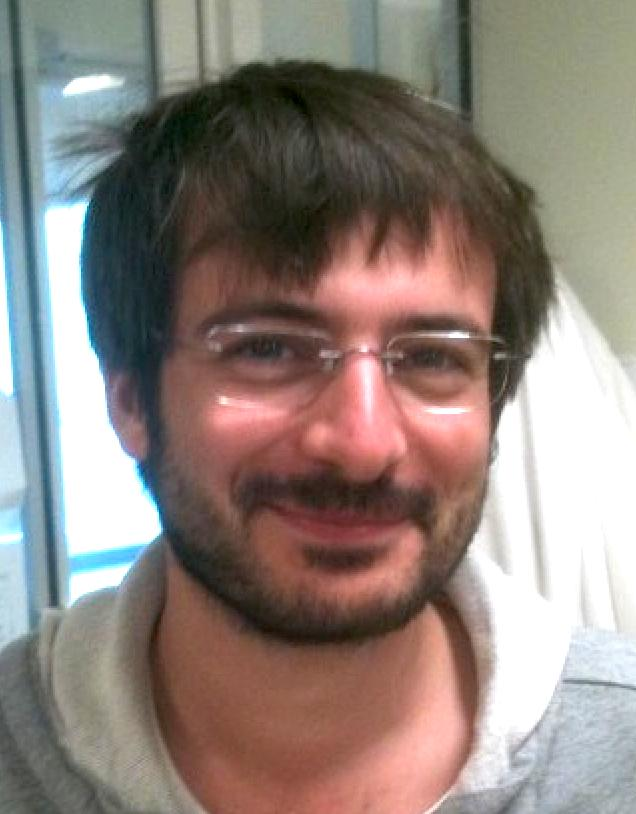
\includegraphics[height=0.3\textheight]{Thibaut}&
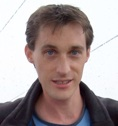
\includegraphics[height=0.3\textheight]{Seb}\\
Christophe Perge & Thibaut Divoux & Sebastien Manneville\\
PhD student & CNRS researcher & Professor\\
E.N.S. Lyon &  CRPP Bordeaux & E.N.S. Lyon\\
\end{tabu}
\end{frame}

\begin{frame}{The yoghurt creep experiment}
\begin{tikzpicture}
\node[anchor=south west] (webcam){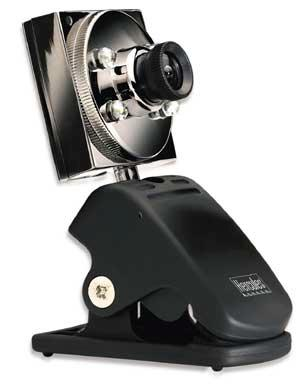
\includegraphics[width=0.2\textwidth]{webcam}};
\node[anchor=south] at (0.4\textwidth,0) (spoon) {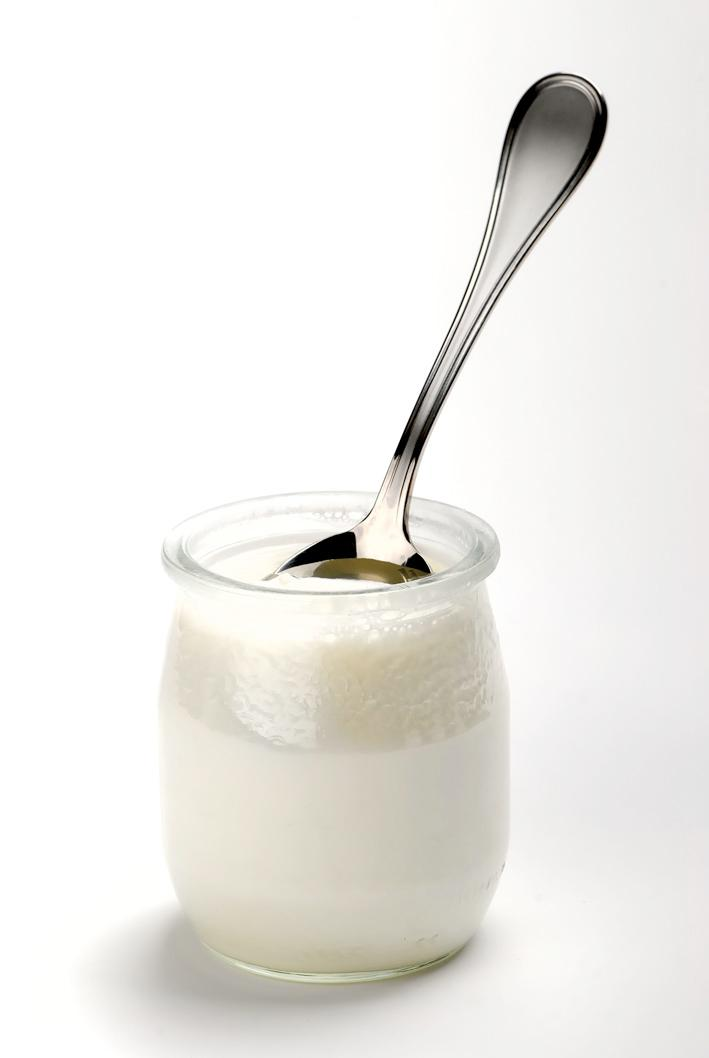
\includegraphics[width=0.3\textwidth]{spoon}};
\node[anchor=south east] at (\textwidth,0) (ultrasound) {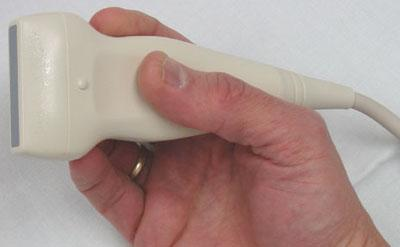
\includegraphics[width=0.4\textwidth]{ultrasound}};

\node[anchor=south west] at ($(ultrasound.north west)+(0,2em)$) (rheometer) {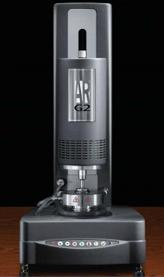
\includegraphics[height=0.4\textheight]{rheometer}};

\begin{scope}[draw]
	\node[below=0of spoon.south] (couette) {A Taylor-Couette cell where the yogurt is made \emph{in situ}};
	\draw[->] (couette) -- ($(spoon.south)+(0,2em)$);
	\node[above=0of ultrasound] {ultrasonic imaging};
	\node[above=0of webcam, text width=0.2\textwidth, align=center] {optical imaging};
	\draw[->] (spoon.north east) +(235:2em) -- (rheometer);
	\node[right=0of rheometer, text width=0.2\textwidth, align=center] {A rheometer imposes a constant stress $\sigma$ and records the strain $\gamma(t)$};
\end{scope}
\end{tikzpicture}
\end{frame}


\section{Wrinkling}

\end{document}

